\section{Einleitung}

\subsection{Motivation}

Bei diesem Versuch geht es darum, Methoden der computergesteuerten Datenaufnahme und -verarbeitung kennenzulernen.
Dazu wird die Biegeschwingung eines Metallstäbchens mithilfe elektronischer Verfahren gesteuert und vermessen.
Solche mechanischen Oszillationen werden oft zur Untersuchung der elastischen Eigenschaften von Festkörpern verwendet.
Die näheren physikalischen Eigenschaften und Ergebnisse spielen in diesem Versuch allerdings eine untergeordnete Rolle.
Es handelt sich jedoch um ein gutes Anwendungsbeispiel computergesteuerter Messaufbauten.

Zudem können wir das verwendete Steuerprogramm für die Messinstrumente, LabVIEW, sowie den für die Kommunikation zwischen PC und Geräten zuständigen General Purpose Interface Bus (GPIB) kennenlernen.
Diese Kombination kann durchaus als ein Standard für computergesteuerte Labormessungen verstanden werden und genießt eine entsprechende Bedeutung.

An die aufgenommenen Daten wird ein theoretisch motiviertes Modell angepasst und somit passende Parameter der Modellierung bestimmt.
Außerdem kann überprüft werden wie gut das Modell die Daten tatsächlich beschreibt.

\subsection{Physikalische Grundlagen}

\subsubsection*{Getriebener gedämpfter harmonischer Oszillator}

Zur theoretischen Beschreibung der verwendeten Biegeschwingung beginnen wir mit der Betrachtung eines durch die periodische Kraft $f_0 \cos \omega t$ getriebenen gedämpften harmonischen Oszillators.
Dessen Differentialgleichung lautet
\begin{align}
\frac{\partial^2 z}{\partial t^2} + \gamma \frac{\partial z}{\partial t} + \omega_0^2 z = f_0 \cos \omega t
\end{align}

mit der Schwingungsamplitude $z$, der Dämpfung $\gamma$ und der Eigenfrequenz der ungedämpften Schwingung $\omega_0$.

Lässt man ein solches System schwingen, ergeben sich nach einem Einschwingvorgang stationäre Lösungen der Form
\begin{align}
    z &= \zeta e^{i(\omega t - \Phi)}
    \\
    \intertext{mit der Phase}
    \label{eq:Phase}
    \tan \Phi &= \frac{\gamma \omega}{\omega_0^2 - \omega^2}
    \\
    \intertext{und der Amplitude}
    \label{eq:Lorentzkurve}
    \zeta &= \frac{f_0}{\sqrt{\left( \omega_0^2 - \omega^2 \right)^2 + \gamma^2\omega^2}}.
\end{align}

Die Sinus- beziehungsweise Cosinus-Anteile der Phase lassen sich mit
\begin{align}
    \label{eq:PhaseSin}
    \sin \Phi &= \frac{\gamma \omega}{\sqrt{ \left( \omega_0^2 - \omega^2 \right) ^2 + \gamma^2 \omega^2}}
    \\
    \intertext{und}
    \label{eq:PhaseCos}
    \cos \Phi &= \frac{\omega_0^2 - \omega^2}{\sqrt{ \left( \omega_0^2 - \omega^2 \right) ^2 + \gamma^2 \omega^2}}
\end{align}

beschreiben. Der Verlauf der Amplituden $\zeta \left( \omega \right)$ in Gleichung \ref{eq:Lorentzkurve} wird als Lorentzkurve bezeichnet.

Der qualitative Verlauf von Phase und Lorentzkurve ist in Abbildung \ref{fig:Lorentzkurve} dargestellt.

\minipage{\linewidth}
    \begin{center}
        \captionsetup{type=figure}
        \begin{adjustbox}{max width=0.45\linewidth, keepaspectratio}
            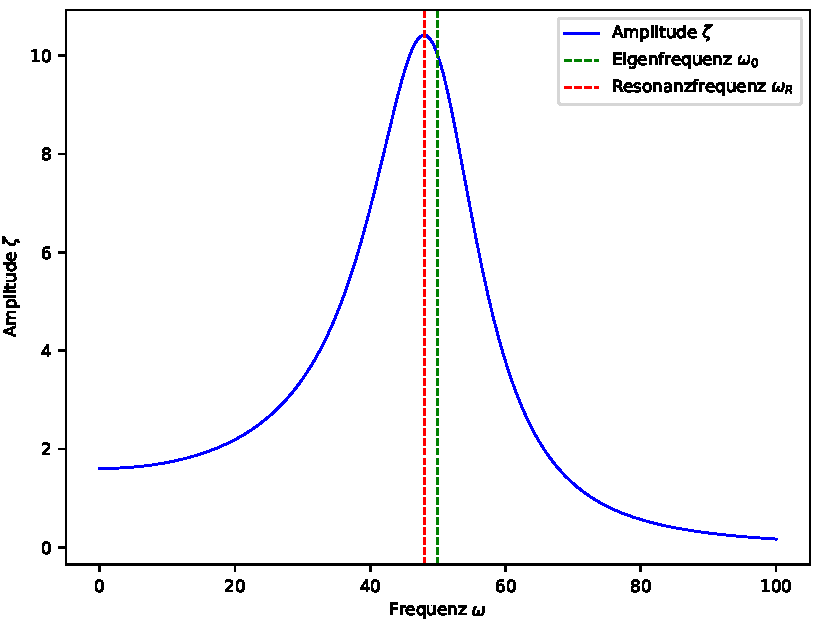
\includegraphics[]{pdf/Lorentzkurve}
        \end{adjustbox}
        \begin{adjustbox}{max width=0.45\linewidth, keepaspectratio}
            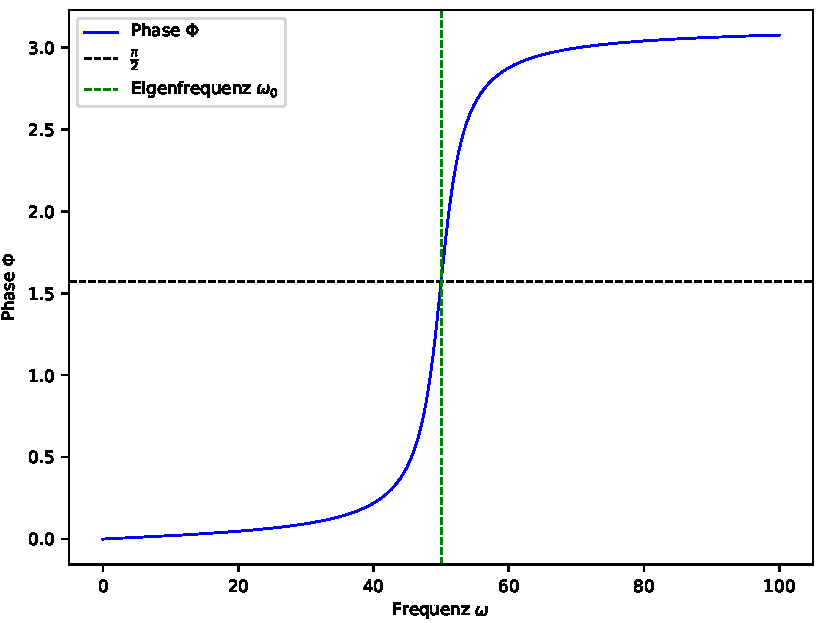
\includegraphics[]{pdf/Phase}
        \end{adjustbox}
        \captionof{figure}{Links: Beispielhafter Verlauf einer Lorentzkurve für $f_0 = 10^7$, $\omega_0 = 50$ und $\gamma = 20$ mit eingezeichneten Werten für Eigenfrequenz $\omega_0$ und Resonanzfrequenz $\omega_R$. Rechts: Beispielhafter Verlauf der Phase für $\omega_0 = 50$ und $\gamma = 5$.}
        \label{fig:Lorentzkurve}
    \end{center}
\endminipage

Im Verlauf der Lorentzkurve erkennt man das charakteristische Resonanzverhalten.
Sie hat ihr Maximum bei der Resonanzfrequenz $\omega_R$:
\begin{align}
    \label{eq:Resonanzfrequenz}
    \omega_R &= \sqrt{\omega_0^2 - \frac{\gamma^2}{2}}.
\end{align}

An der Phase ist zu erkennen, dass die Oszillatorschwingung hinter der Anregung her schwingt, im Resonanzfall genau um $\frac{\pi}{2}$ verzögert.

Die Ausprägung des Peaks der Lorentzkurve ist abhängig von der Dämpfung $\gamma$ des Oszillators.
Je kleiner $\gamma$, desto ausgeprägter ist der Peak.

Als Maß hierfür definieren wir die Güte
\begin{align}
    \label{eq:Guete}
    Q = \frac{\omega_0}{\gamma} = 2 \pi \frac{E}{|\Delta E|}.
\end{align}

Diese gleicht dem Energieverlust pro Schwingung eines theoretischen ungetriebenen Oszillators mit sonst gleichen Eigenschaften.

\subsubsection*{Harmonische Wellen}

Breitet sich eine Schwingung in Raum und Zeit aus, so entsteht eine Welle.
Eine harmonische Welle die sich in $x$-Richtung ausbreitet wird beschrieben durch
\begin{align*}
    \frac{\partial^2 z}{\partial t^2} &= v_\mathrm{ph}^2 \; \frac{\partial^2 z}{\partial x^2}.
\end{align*}

Dabei ist $z$ die Auslenkung und $v_\mathrm{ph}$ Phasengeschwindigkeit der Welle.

Wenn der Raum in dem sich die Welle ausbreiten kann durch Randbedingungen beschränkt ist ergibt sich eine stehende Welle.
Die Welle wird an einer Berandung reflektiert und die ausfallende Welle überlagert sich mit der einfallenden.\\
Ist eine eindimensional schwingendes System etwa bei $x=0$ und $x=l$ eingespannt, die Amplitude also immer Null, so gilt für die Wellenlängen der entstehenden Welle:
\begin{align}
    \lambda_n &= \frac{2l}{n}, \hspace{1cm} n=1,2,3,...
\end{align}

Diese stehenden Wellen können als Eigenschwingungen des Systems betrachtet werden.
Deren Frequenzen
\begin{align}
    \nu_n = \frac{v_\mathrm{ph}}{\lambda_n} = \frac{v_\mathrm{ph} n}{2 l}
\end{align}

sind ganzzahlige vielfache der Grundfrequenz $\nu_0$ und werden als Oberschwingungen bezeichnet.

\subsubsection*{Erzwungene gedämpfte Biegeschwingung eines elastischen Reeds}

Im Versuch benutzen wir die elastische Biegeschwingung eines metallenen Reeds.
Die genaue mathematische Herleitung der Differentialgleichung dieses Systems ist sehr umfangreich.
Dafür verweisen wir auf die in der Versuchsanleitung \cite{Anleitung} bereits eingeführte Diplomarbeit \cite{Diplomarbeit} von Johannes Claßen.
Hier geben wir lediglich das Ergebnis und die sich daraus ergebenden Konsequenzen für unser Experiment an.
Die transversale Auslenkung $z$ eines kleinen Teil des Reeds an der Position $x$ wird durch
\begin{align}
    \frac{\partial^2 z}{\partial t^2} + \frac{d^2}{12} v_{\Upsilon}^2 \frac{\partial^4 z}{\partial x^4} = f_0 e^{i \omega t} \delta(x-l)
\end{align}

bestimmt.
Dabei sind $d$ und $l$ die Dicke und Länge des Reeds und $v_{\Upsilon} = \sqrt{\frac{E}{\rho}}$ die Schallgeschwindigkeit im Reed.

Auch diese Schwingung zeigt Resonanzverhalten und lässt sich um die Maxima herum durch die Lorentzkurve approximieren.

Die diskreten Eigenfrequenzen liegen bei
\begin{align}
    \label{eq:Eigenfrequenzen}
    \nu_n &= \alpha_n (2n+1)^2 \frac{\pi}{16\sqrt{3}} \frac{d}{l^2} v_{\Upsilon}
    \intertext{mit den numerischen Konstanten}
    \alpha_0 = 1,424987 \hspace{0.5cm} \alpha_1 &= 0,992249 \hspace{0.5cm} \alpha_2 = 1,000198
\end{align}

Damit ergeben sich feste Frequenzverhältnisse zwischen den verschiedenen Schwingungsmoden
\begin{align}
    \frac{\nu_1}{\nu_0} = 6.267
    \hspace{0.5cm}
    \frac{\nu_2}{\nu_0} = 17.548
    \label{eq:VerhaeltnisseEingenfrequenzen}
\end{align}

\subsection{Messung am experimentellen Aufbau}

Der schematische Aufbau des Experiments ist in Abbildung \ref{fig:SchemaVersuchsaufbau} dargestellt.

Für den schematischen Aufbau des Experiments verweisen wir an die Versuchsanleitung \cite{Anleitung}.
\todo{Bild aus dem Seminar-Vortrag einfügen oder eben nicht - und dann entsprechend einen der beiden Sätze löschen.}

Um einen wichtigen Aspekt für die spätere Auswertung der Messdaten zu erkennen, ist es nötig, sich die Beziehung der wirkenden Kraft herzuleiten.
Als Grundlage der Herleitung verwenden wir die Kraft zwischen zwei Kondensatorplatten:
\begin{align}
    \label{eq:KraftKondensatorplatten}
    \begin{split}
        F = \frac{C_a U^2}{2 g_a}
    \end{split}
\end{align}

Mithilfe der Kapazität der Anregungselektrode
\begin{align}
    \label{eq:KapazitaetAnregungselektrode}
    \begin{split}
        C_a = \frac{\varepsilon_0 S}{g_a}
    \end{split}
\end{align}

und einer angelegten Wechselspannung $U(t) = U_0 \cos \omega t$ erhalten wir schließlich die periodische Kraft, welche unsere Schwingung anregt
\begin{align}
    \label{eq:PeriodischeKraft}
    \begin{split}
        F \left( t \right) = \frac{C_a {U_0}^2}{4 g_a} \left( 1 + \cos 2 \omega t \right).
    \end{split}
\end{align}

Wir erkennen: \textbf{Die Frequenz der Schwingung wird doppelt so groß sein wie die eingestellte Frequenz unseres Erregers.}

Analog lässt sich über die Kapazität der Detektionselektrode
\begin{align}
    \label{eq:KapazitaetDetektionselektrode}
    \begin{split}
        C_d = \frac{\varepsilon_0 S}{g_d}
    \end{split}
\end{align}

eine Beziehung zwischen Schwingung und gemessener Spannung herleiten.
Die Spannung der Detektionselektrode lässt sich schließlich schreiben als
\begin{align}
    \label{eq:Detektionselektrode}
    \begin{split}
        U_d &= U_B \frac{z}{g_d} \frac{C_d}{C_d + C_L} \frac{\omega R \left( C_d + C_L \right)}{\sqrt{1+\left( \omega R \left( C_d + C_L \right) \right)^2}}
    \end{split}
\end{align}

wobei wir uns zunächst von der Frequenzunabhängigkeit des Übertragungsverhältnisses $\left| \frac{U_d}{z} \right|$ überzeugen möchten.

Dazu kann für den im Experiment verwendeten Frequenzbereich von $\frac{\omega}{2\pi} > \SI{100}{\hertz}$ der letzte Faktor in Gleichung \ref{eq:Detektionselektrode} (entspricht Gleichung 2.6 der Versuchsanleitung \cite{Anleitung}) in guter Näherung durch \SI{1}{} ersetzt werden.
Der Verlauf des Faktors in Abhängigkeit von $\omega$ ist in Abbildung \ref{fig:Faktor} dargestellt.

\minipage{\linewidth}
    \begin{center}
        \captionsetup{type=figure}
        \begin{adjustbox}{max width=\linewidth, keepaspectratio}
            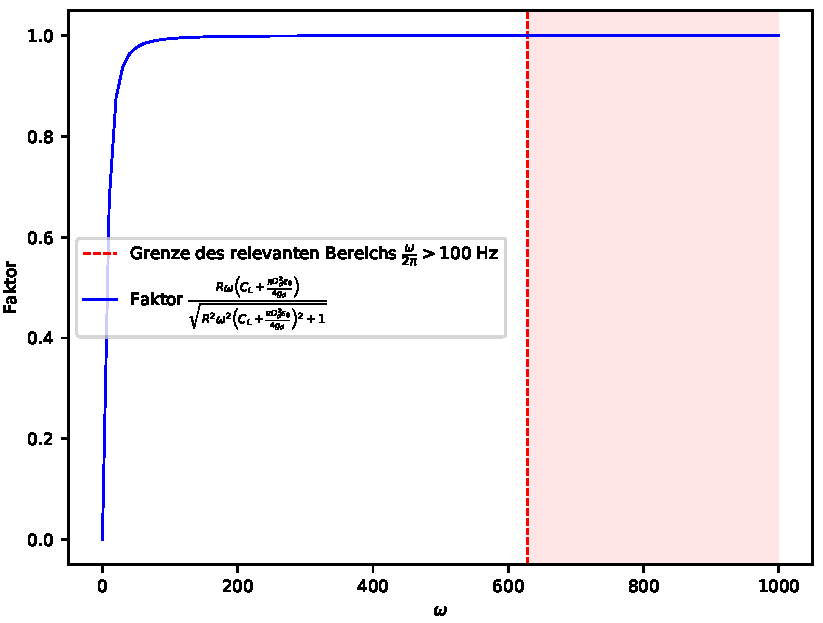
\includegraphics[]{pdf/Faktor}
        \end{adjustbox}
        \captionof{figure}{Letzter Faktor in Gleichung \ref{eq:Detektionselektrode} (entspricht Gleichung 2.6 der Versuchsanleitung \cite{Anleitung}) kann in guter Näherung durch \SI{1}{} ersetzt werden.}
        \label{fig:Faktor}
    \end{center}
\endminipage

Außerdem stellen wir fest, dass $C_d \ll C_L$ und können somit insgesamt schreiben
\begin{align}
    \label{eq:DetektionselektrodeVereinfacht}
    \begin{split}
        U_d &\approx U_B \frac{z}{g_d} \frac{C_d}{C_L}
    \end{split}
\end{align}

Diese Beziehung lässt sich also dazu verwenden, zu den im Experiment gemessenen Werten für $U_d$ die entsprechende Auslenkung $z$ der Schwingung zu berechnen.

\subsection{Einige Abschätzungen zur Vorbereitung}

Um uns die Dimensionen des Experiments deutlich zu machen, berechnen wir nun den erwarteten Maximalwert des Amplitudenverlaufs $\zeta$.
Wir nutzen Gleichung 2.8 der Versuchsanleitung
\begin{align}
    \label{eq:MaximaleAmplitude}
    \begin{split}
        \zeta_0 = 4 \frac{l^3}{Ed^3b} F_0
    \end{split}
\end{align}

wobei $F_0$ der Maximalwert der periodischen Anregungskraft nach Gleichung \ref{eq:PeriodischeKraft} ist.

Damit lässt sich nun auch der Maximalwert der Spannung der Detektionselektrode $U_d$ nach Gleichung \ref{eq:DetektionselektrodeVereinfacht} bestimmen.
Wir erhalten die beiden Werte $\zeta_0 = \SI{2.55}{\nano\meter}$ und $U_{d0} = \SI{5.76}{\micro\volt}$.

\textbf{Die abgeschätzten Größenordnung unserer Messgrößen bestätigen also die Notwendigkeit des Verstärkers.}

\subsection{Theoretische Werte für die erwarteten Eigenfrequenzen}

Mithilfe Gleichung \ref{eq:Eigenfrequenzen} und den Angaben zum Reed in der Versuchsanleitung \cite{Anleitung} lassen sich die erwarteten Eigenfrequenzen abschätzen.
Das erleichtert uns die spätere Suche nach den tatsächlichen Resonanzkurven während des Experiments.

Wir erhalten $\nu_{0 theo} = \SI{274}{\hertz}$, $\nu_{1 theo} = \SI{1719}{\hertz}$ und $\nu_{2 theo} = \SI{4812}{\hertz}$.
\label{eq:AbschaetzungEigenfrequenzen}

\subsection{Statistische Grundlagen}

Eine Einführung in die statistischen Grundlagen, die wir beispielsweise als Basis zur Erstellung der Fits an die Messdaten verwendet haben, würde den Umfang dieses Texts sprengen.
Wir verweisen daher an dieser Stelle an die entsprechenden Kapitel der Versuchsanleitung \cite{Anleitung}.
